% Parent preamble: \usepackage{graphicx,amsmath} (and caption/booktabs if floats are customized).
\subsection{Pseudopotential Kohn--Sham discretization convergence}

We now verify the accuracy and performance of SPARC-atomSFE for pseudopotential Kohn--Sham DFT calculations. Unless otherwise specified, we use an exponential mesh with shift $c=0$, concentration parameter $a=20$, domain size $R_{max}=40$~Bohr, $N_{fe}=10$ finite elements, polynomial degree $p=20$, and quadrature order $q=60$. We employ the SPMS suite of ONCV pseudopotentials, which include nonlinear core corrections.

We begin by studying convergence with respect to the domain size $R_{max}$ and the number of finite elements $N_{fe}$. In particular, Figure~\ref{fig:psp-gga-pbe-convergence} shows the convergence of the total energy and occupied valence eigenvalues for the PBE functional across atoms with atomic numbers $Z=1$--$57$ and $Z=72$--$83$, with reference results computed using $R_{max}=40$~Bohr and $N_{fe}=16$. We observe that both quantities converge exponentially with increasing $R_{max}$, with errors below $10^{-6}$~Ha achieved at $R_{max}\sim 27$~Bohr. We also observe rapid convergence with increasing $N_{fe}$, with accuracies better than $10^{-6}$~Ha attained at $N_{fe}\sim 9$. These results are consistent with previous GGA results obtained using a spectral scheme based on Chebyshev polynomials. We also find similar convergence behavior for all other exchange-correlation functionals considered here, with the exception of RPA-OEP, which has not been tested in the pseudopotential context.

\begin{figure}[!htbp]
    \centering
    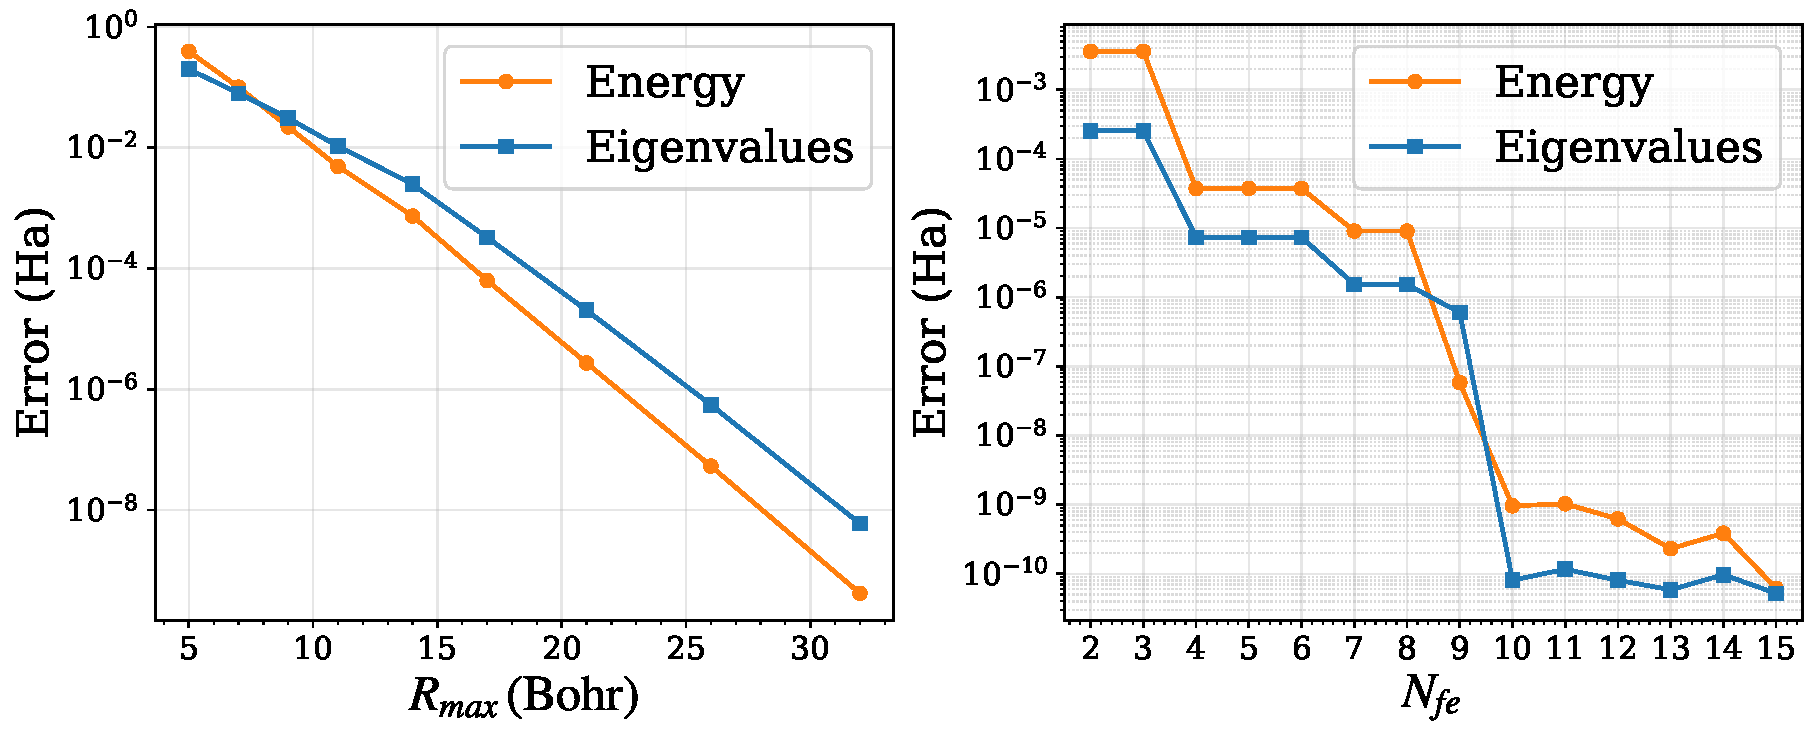
\includegraphics[width=\textwidth]{../figures/pseudo_gga_pbe_convergence_test_summary}
    \caption{Convergence of the total energy and occupied valence eigenvalues with respect to domain size $R_{max}$ (left) and number of finite elements $N_{fe}$ (right) in pseudopotential Kohn--Sham DFT calculations, using the PBE exchange-correlation functional, for atomic numbers $Z=1$--$57$ and $Z=72$--$83$. The energy error is defined as the maximum absolute total-energy difference over all atoms in the set, while the eigenvalue error is defined as the maximum, over those atoms, of the per-atom mean absolute difference in the occupied valence eigenvalues. Reference values are computed using domain size $R_{max}=40$~Bohr and $N_{fe}=16$ finite elements.}
    \label{fig:psp-gga-pbe-convergence}
\end{figure}

As supplementary material to the convergence discussion presented in the main paper, the pseudopotential sweeps likewise use \emph{nested} subsets of a common reference exponential mesh, rather than regenerating independent meshes for each choice of $R_{max}$ or $N_{fe}$. This construction isolates the effect of radial resolution while preserving the underlying exponential mesh distribution across discretization levels. Figure~\ref{fig:psp-boundary-subset-rule} illustrates this subset construction for the pseudopotential case.

\begin{figure}[!htbp]
    \centering
    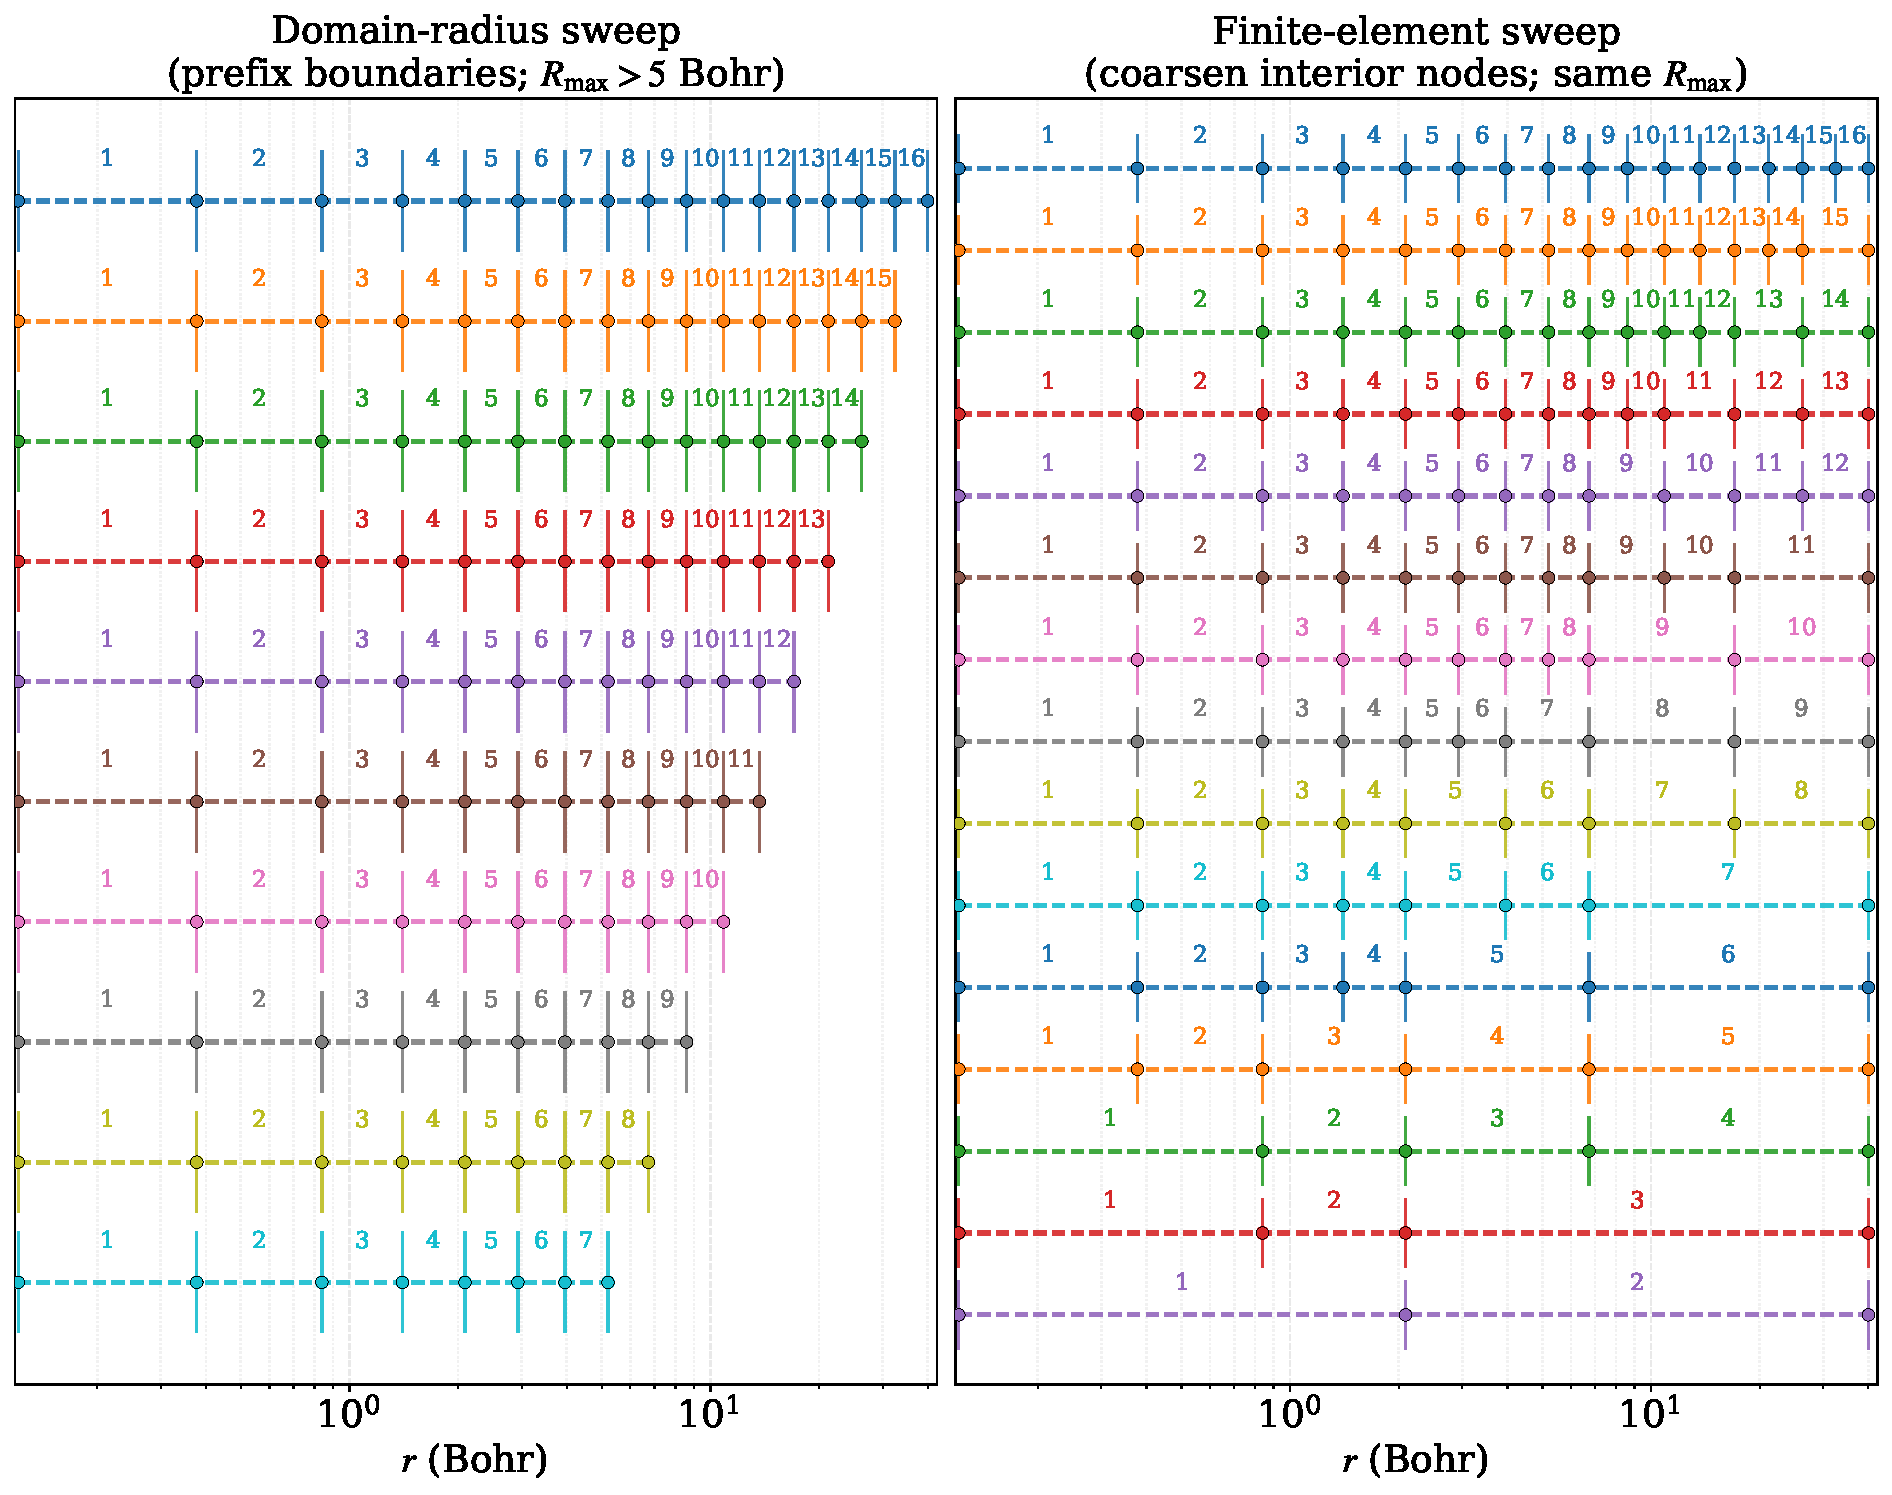
\includegraphics[width=\textwidth]{../figures/boundary_subset_rule_psp}
    \caption{Nested radial mesh subsets used in pseudopotential convergence sweeps: each coarser level retains node locations inherited from the reference exponential mesh, so only resolution changes—not the global mesh law.}
    \label{fig:psp-boundary-subset-rule}
\end{figure}

Finally, Figures~\ref{fig:psp-lda-svwn-convergence} and~\ref{fig:psp-rscan-convergence} give LDA-SVWN and rSCAN counterparts to Figure~\ref{fig:psp-gga-pbe-convergence}: the same two-panel layout, error definitions, reference mesh ($R_{max}=40$~Bohr, $N_{fe}=16$), and atom ranges $Z=1$--$57$ and $Z=72$--$83$, with discretization trends consistent with the PBE panels in Figure~\ref{fig:psp-gga-pbe-convergence}. Together with the mesh construction recorded above, these results provide additional numerical evidence for the pseudopotential convergence picture presented in the main paper.

\begin{figure}[!htbp]
    \centering
    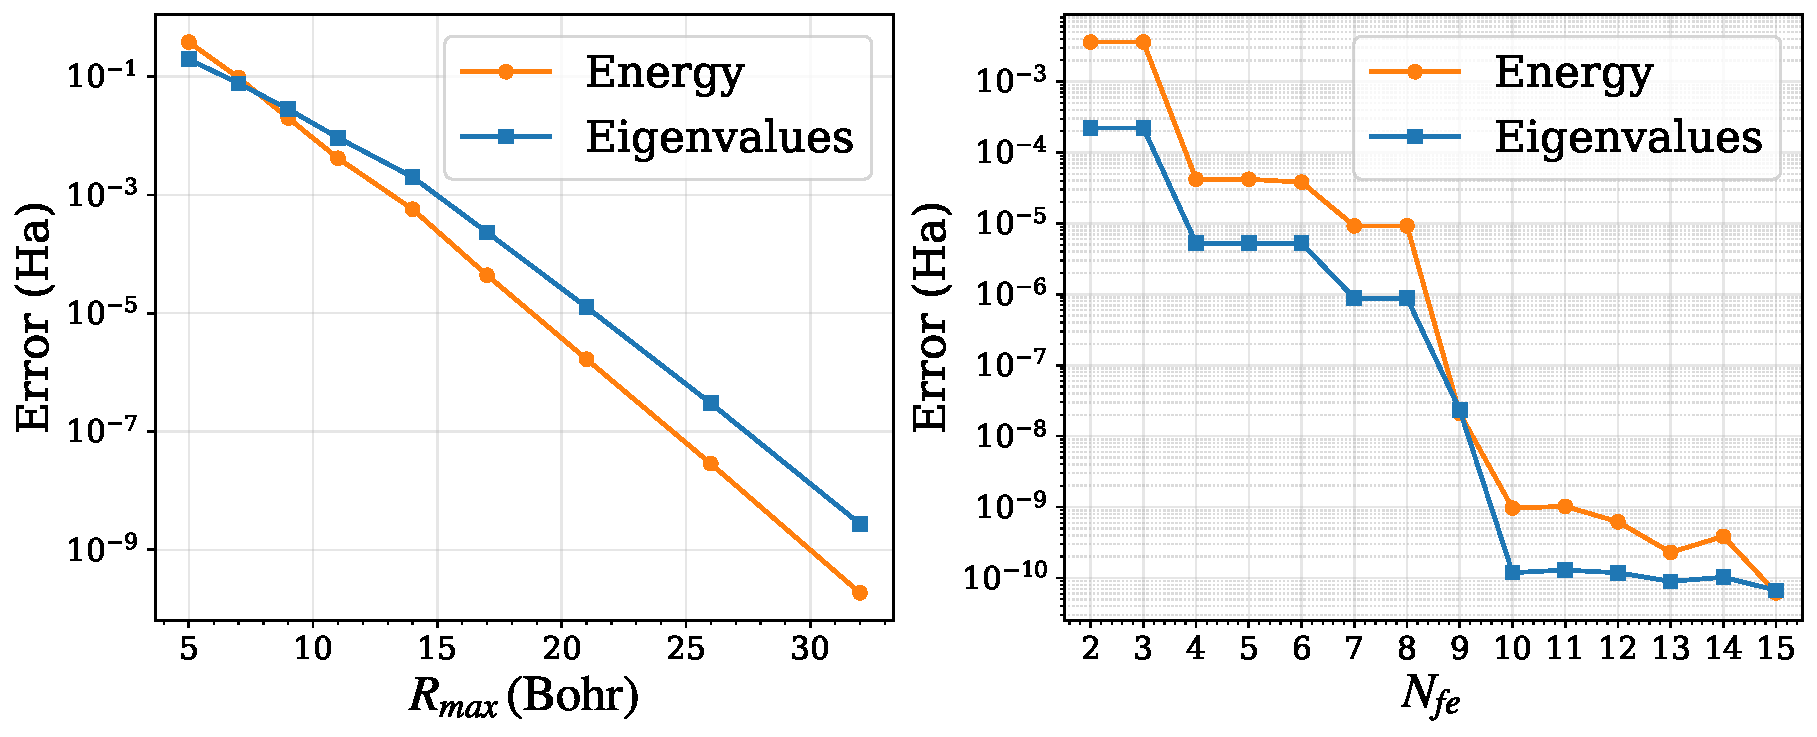
\includegraphics[width=\textwidth]{../figures/pseudo_lda_svwn_convergence_test_summary}
    \caption{Same as Figure~\ref{fig:psp-gga-pbe-convergence}, for the LDA-SVWN exchange-correlation functional.}
    \label{fig:psp-lda-svwn-convergence}
\end{figure}

\begin{figure}[!htbp]
    \centering
    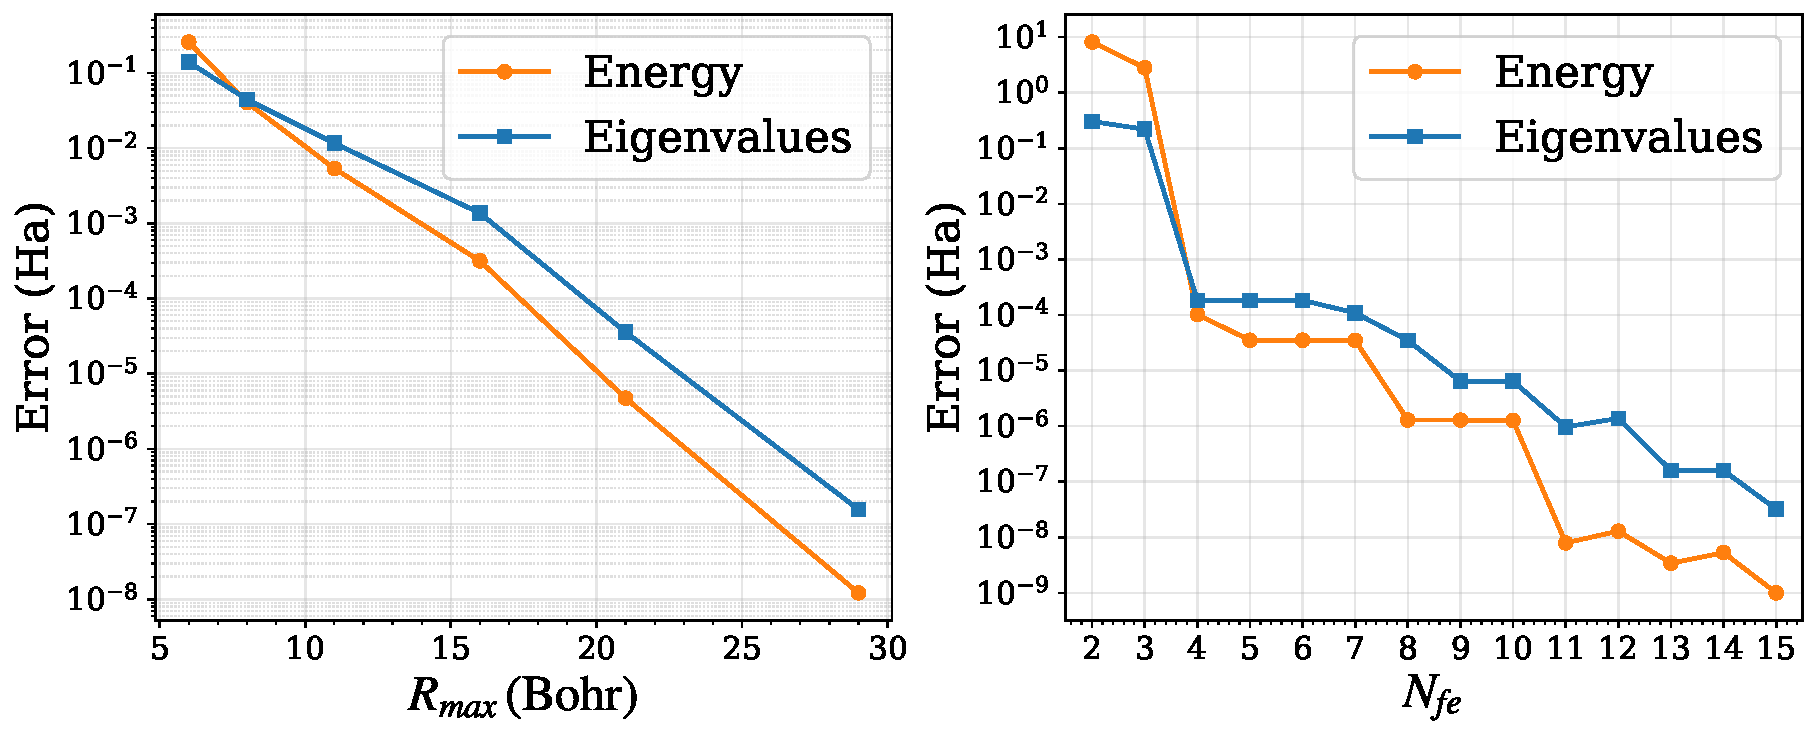
\includegraphics[width=\textwidth]{../figures/pseudo_rscan_convergence_test_summary}
    \caption{Same as Figure~\ref{fig:psp-gga-pbe-convergence}, for the rSCAN meta-GGA exchange-correlation functional.}
    \label{fig:psp-rscan-convergence}
\end{figure}
